
\documentclass[12pt]{article}

\usepackage{graphicx}
\usepackage[margin=1in]{geometry}
\usepackage{microtype}
\usepackage{listings}
\usepackage{hyperref}
\usepackage[monochrome]{color}
\usepackage{xcolor}

\hypersetup{colorlinks=true}

\title{Data Visualization Workshop \\ ``Seeing and Knowing in Astronomy and Art''}
\author{Asher Wasserman \\ email: \href{mailto:adwasser@ucsc.edu}{adwasser@ucsc.edu}}
\date{May 21, 2016}

\begin{document}

\maketitle

\section{Outline}
\label{sec:outline}
Much of this workshop has focused on how astronomy has historically been done.  Astronomers rarely draw by hand what they see anymore, in part due to the challenges of accurately representing increasingly complex (and in some cases multi-dimensional) images.  In this activity, we'll have a brief introduction to modern astronomical data visualization with \emph{SAOImage DS9}.  The low-level (i.e., technical) goal for the exercise is to get comfortable opening and viewing images with this particular software.  The high-level (i.e., abstract) goal is to understand how choices in data visualization influence how we do scientific inference in astronomy.

Section~\ref{sec:req} describes how to install ds9 and obtain the image files we'll be using.  Section~\ref{sec:start} will work on getting familiar with moving around and changing the intensity scale for a single image.  Section~\ref{sec:multiple} will work on how to compare features between images at the same spatial positions.  Section~\ref{sec:color} is a short tutorial on making color-composite images.  Section~\ref{sec:spec} will work on interpreting spatial resolved spectra from a radio interferometer, a much different dataset than the those investigated in the previous sections.  Sections~\ref{sec:color} and \ref{sec:spec} are independent of each other, but the previous two should be completed before moving on.  Section~\ref{sec:synth} asks you to put the activity in context with the rest of the workshop.  Do as much as you have time for, and don't be afraid to play around with anything interesting you find!

\section{Requirements}
\label{sec:req}

You'll need a computer with a modern operating system (Linux, Mac OSX, or Windows 7/8/10).  We will
be using \emph{SAOImage DS9} (here on out just called ds9), an open source scientific software package, 
to display images stored as FITS files.  The program is available for download at \url{http://ds9.si.edu/site/Download.html}.  Choose the appropriate one for your operating system.  For Mac this should be an application which can be dragged into your Applications folder.  For Windows, this should be an executable that unzips files into a folder called ds9.  This folder should then have an executable file called ``ds9.exe''.  Double clicking on this file should open a window similar to the one shown below.  If you have any issues running ds9, email me for assistance.

\begin{figure}[h]
  \centering
  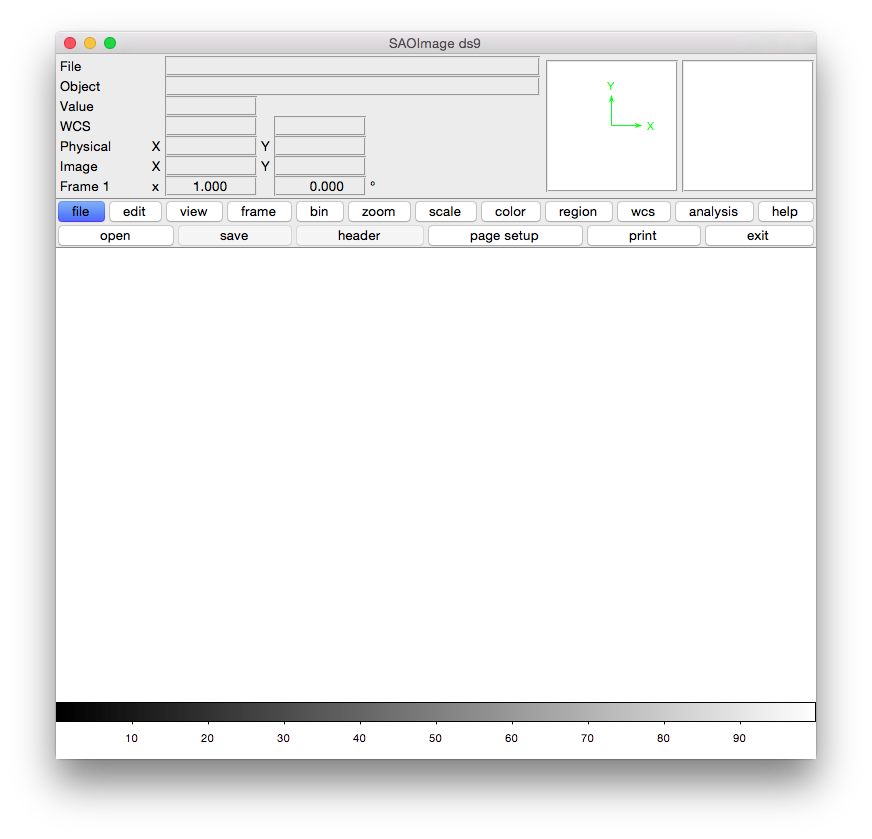
\includegraphics[width=0.6\linewidth]{ds9_screenshot.png}
  \caption{DS9 opening screen on a Mac installation.}
  \label{fig:open}
\end{figure}

In addition to the software, it would be helpful to download some image files ahead of time.  We will be looking at FITS (Flexible Image Transport System) files.  The files are available for download here:
\url{https://drive.google.com/folderview?id=0B1C3GCppwoesSllacTNnemtvTm8&usp=sharing}.  They may be compressed (e.g., a zip file), in which case the file extension will be \texttt{.fits.gz} instead of \texttt{.fits}.  You do not need to unzip the files; ds9 will interpret this automatically for you.

\section{Starting out}
\label{sec:start}

Open ds9 (you should be able to just double-click on the downloaded executable file).  Go to \texttt{File -> Open} and select the file \texttt{m83\_dss\_ir.fits} from the window that pops up. %(fig~\ref{fig:open})
You may need to navigate to where you saved the downloaded image file by choosing which directory you are in.  This is done by clicking in the Directory box on the right side of the window.  If you need to go up by a folder, click on the double dots (\texttt{..}) 

% \begin{figure}[h]
%   \centering
%   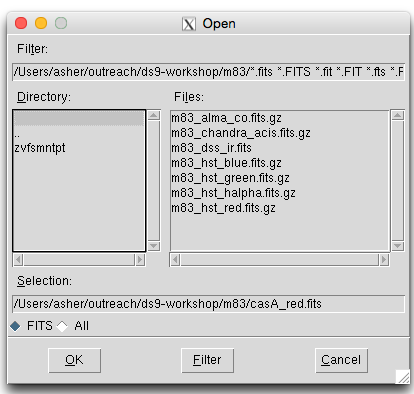
\includegraphics[width=0.6\linewidth]{open_screen.png}
%   \caption{DS9 file open window.}
%   \label{fig:open}
% \end{figure}

Once the image appears, try moving around.  There are options in the menubar to zoom in and out.  To pan around with the mouse, click on \texttt{Edit -> Pan}.  You can also zoom with the mouse wheel and pan with the middle mouse button (if it exists).  If you manage to get lost, you can get back to where you were by clicking on \texttt{Zoom -> Center Image} and \texttt{Zoom -> Zoom to Fit Frame}.  

As you move your cursor along in the image, some numbers written out on the top of the image window should change.  What do these numbers represent?  How do they change as you move the cursor?

The image we're looking at is of Messier 83, a barred spiral galaxy, taken from the Digitized Sky Survey, a digital archive of photographic plates.  This one in particular was taken with the UK Schmidt Telescope at the Anglo-Australian Observatory.

Let's investigate how ds9 is interpreting what this image should look like.  Open up the Scale Parameters window by clicking on \texttt{Scale -> Scale Parameters}.  You should see something that looks like fig.~\ref{fig:scale}.  The histogram plotted in this window shows the distribution of pixel brightness values in the image.  Based on the histogram, are there more bright or dim pixels?

\begin{figure}[h]
  \centering
  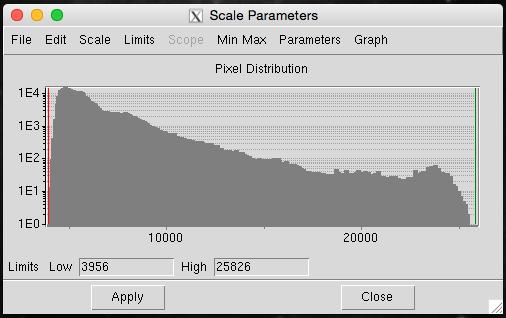
\includegraphics[width=0.6\linewidth]{scale.png}
  \caption{DS9 scale parameters window.}
  \label{fig:scale}
\end{figure}

The way ds9 represents an image is by mapping brightness values of pixels to an intensity value (represented by the color bar on the bottom of the image window).  In the default setting, this color map goes from black to white.  The lower and upper limits in the scale parameters window show what pixel values will be mapped to black and white respectively, with in-between pixel values given linearly increasing intensities.  Any pixel values above the upper limit will all be mapped to pure white and any pixel values below the lower limit will be mapped to pure black.  Try experimenting with these settings.  You can either click and drag the red and green bars on either side of the histogram or type in numbers below the histogram (in which case click apply to make changes).  To reset to the original scale, click on \texttt{Limits -> Min Max}.  What sort of features get highlighted or ignored based on the scale settings you choose?

\section{Working with multiple images}
\label{sec:multiple}

Let's look at another image of this object taken from a more modern telescope.  Click on \texttt{Frame -> New Frame}.  The display should clear.  Now go to \texttt{File -> Open} and select \texttt{m83\_hst\_halpha.fits.gz}.  Your color scale will probably be set from the previous image.  Play around with the color scale settings as you did for the previous image to find some thing that works nice.

Now we want to compare this image with the previous image and convince ourselves that it is indeed the same image.  When we made a new frame and opened the new image, we didn't actually get rid of the old one.  Click on \texttt{Frame -> Tile Frames} to see this.  Now we need to match the spatial (zoom) scales.  You might have noticed that ds9 can keep track of a world coordinate system (WCS) like the spatial coordinates of right ascension (RA) and declination (Dec).  To match the coordinates between the two images, go to \texttt{Frame -> Lock -> Frame} and click on \texttt{WCS}.  This action will force images to align to their world coordinates whenever a change, such as panning or zooming, occurs.  You'll notice that you can lock various viewing features across all images loaded into ds9, such as the colorbar and the intensity scaling.

One other tool that you may find useful in convincing yourself that these are in fact the same object is the crosshairs.  You can get this tool from \texttt{Edit -> Crosshair}, and then clicking the left mouse button will allow you to move the crosshairs.  To match the crosshairs between the two images, go to \texttt{Frame -> Lock -> Frame -> Crosshair}.

What are the differences between the two images?  Which has a wider field of view, and which has better spatial resolution?  Are there overlapping features?  Are there features that appear in one which don't appear in the other? 

The higher spatial resolution we have been looking at was taken with a narrow-band filter on the Hubble Space Telescope.  This photometric band captures the H$\alpha$ (pronounced ``aitch alpha'') emission line, which is often seen in star-forming regions.  Try looking at the other ``colors'' taken with the Hubble Space Telescope (\texttt{m83\_hst\_red.fits.gz}, \texttt{m83\_hst\_green.fits.gz}, \texttt{m83\_hst\_blue.fits.gz}), and comparing their features.  More on this in the next section!

\section{Color-composite images}
\label{sec:color}

Throughout the past few sections, we've been viewing images in greyscale (or some other monotonic intensity map if you've played around with the choice of colormap).  But what about all those nice images we see from the Hubble Space Telescope?  In general, those are all color-composite images, produced by making a balance of red, green, and blue images added together.  Let's try making one for ourselves.  

To clear all frames, click on \texttt{Frame -> Delete All Frames}.  Now make a different type of frame by clicking on \texttt{Frame -> New Frame RGB}.  You should have the color bar indicator on the bottom show red, green, and blue scales instead of the grey scale which was there for a regular frame.  There should also be a new small window that pops up which looks like fig.~\ref{fig:rgb}. This window has a radio button for selecting which color is being edited, and toggle buttons for selecting which color frames are visible. 

\begin{figure}[h]
  \centering
  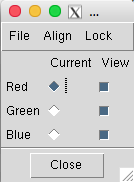
\includegraphics[width=0.3\linewidth]{rgb.png}
  \caption{DS9 RGB frame window}
  \label{fig:rgb}
\end{figure}

With the Current frame set to Red, open (\texttt{File -> Open}) the image \texttt{m83\_hst\_red.fits.gz}.  It should appear on the frame with a red color bar.  Now set the Current frame to Green, and open \texttt{m83\_hst\_green.fits.gz}.  To see what this image looks like by itself, toggle the Red frame so that it is no longer visible.  Finally, set the Current frame to Blue and open \texttt{m83\_hst\_blue.fits.gz}.  Note that each color frame has it's own intensity scale settings.  Play around with different scalings in each color.

While we chose to represent each HST image with colors roughly corresponding to the wavelength range they were taken in, there's no reason we have to do this.  You could just as easily make a false color image using different inputs.  Try swapping out the Red frame for the H$\alpha$ image we were looking at earlier.  What features immediately jump out?

If you want to try making a color composite image of an entirely different object, check out the images of Cassiopeia A (\texttt{casA\_red.fits}, \texttt{casA\_green.fits}, and \texttt{casA\_blue.fits}), taken with the Chandra X-ray Observatory.  These images don't correspond to optical colors that we are used to, but rather to different energies of X-rays.

\section{Spatially resolved spectra}
\label{sec:spec}

For this last part, we're going to look at a different type of data, taken the Atacama Large Millimeter/Sub-millimeter Array (ALMA) a radio interferometer array.  Open the file \texttt{m83\_alma\_co.fits.gz}.  When you do so, the Cube window should pop up (fig.~\ref{fig:cube}).  If not, you can open this window by clicking on \texttt{Frame -> Cube}.  You'll notice that initially, this image seems to be completely blank, despite your best efforts to scale the intensity by different amounts.  To go through slices (or layers) in this cube, you can either drag the top slider in the Cube window or click Next in the Cube window.  The Play button will cycle through slices one by one, and the speed can be set with the Interval setting at the top of the window.  Cycle through the cube to see what it contains.

The data we are looking at is a molecular line transition of carbon monoxide, which is a good tracer of molecular gas mass. Each slice of the cube represents emission at a particular frequency of radio waves.  Since a frequency shift from the center of line location can be caused by motion along the line-of-sight between us and the gas (think back to the Doppler effect from physics), each slice can also be thought of as the emission of gas traveling at a particular line-of-sight velocity.

In light of this physical interpretation, what can you say about the distribution of the gas?  Try comparing this image with the H$\alpha$ image we were looking at earlier.  Are there places where the molecular gas emission lines up with the H$\alpha$ emission (tracing ionized hydrogen)?

\begin{figure}[h]
  \centering
  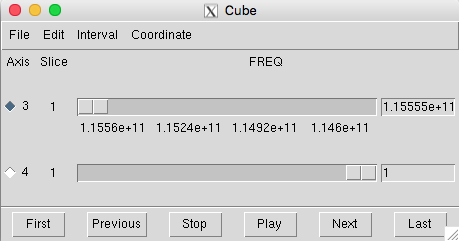
\includegraphics[width=0.6\linewidth]{cube.png}
  \caption{DS9 cube window}
  \label{fig:cube}
\end{figure}

\section{Synthesis questions}
\label{sec:synth}

\begin{itemize}

\item What choices did you have in presenting a single-color image?  How did these choices affect what you observed?  Were there trade-offs in these choices, or could you find some settings that did everything you wanted?

\item When comparing images of the same object in different parts of the spectrum, did you find it more useful to make a color-composite, or to put them in separate grey scale frames?  What are the features that get put into the viewer's focus in each color image?  Is the focus clearer, or harder to discern, when comparing in a color-composite as compared to separate grey scale images?

\item Does the visualization process change depending on what you see as being in the foreground as opposed to the background?  While these terms can have a physical meaning in terms of distance from the viewer, how do these terms relate to the creation of an image?

\item What are some ways you could represent the multi-dimensional radio data from the last section in conjunction with the two-dimensional optical view from Hubble?

\item Can you think of ways in which you could be misleading about how you present a data visualization?

\item Are there objective principles for presenting data, or do we need to accept that it is a subjective process (and just make sure we communicate our process well)?

\end{itemize}

\end{document}

%%% Local Variables:
%%% mode: latex
%%% TeX-master: t
%%% End:
